% Editable native annotations around unchanged verified IDE photographs.
\par
\begin{figure}[htbp]
\centering
\sbox0{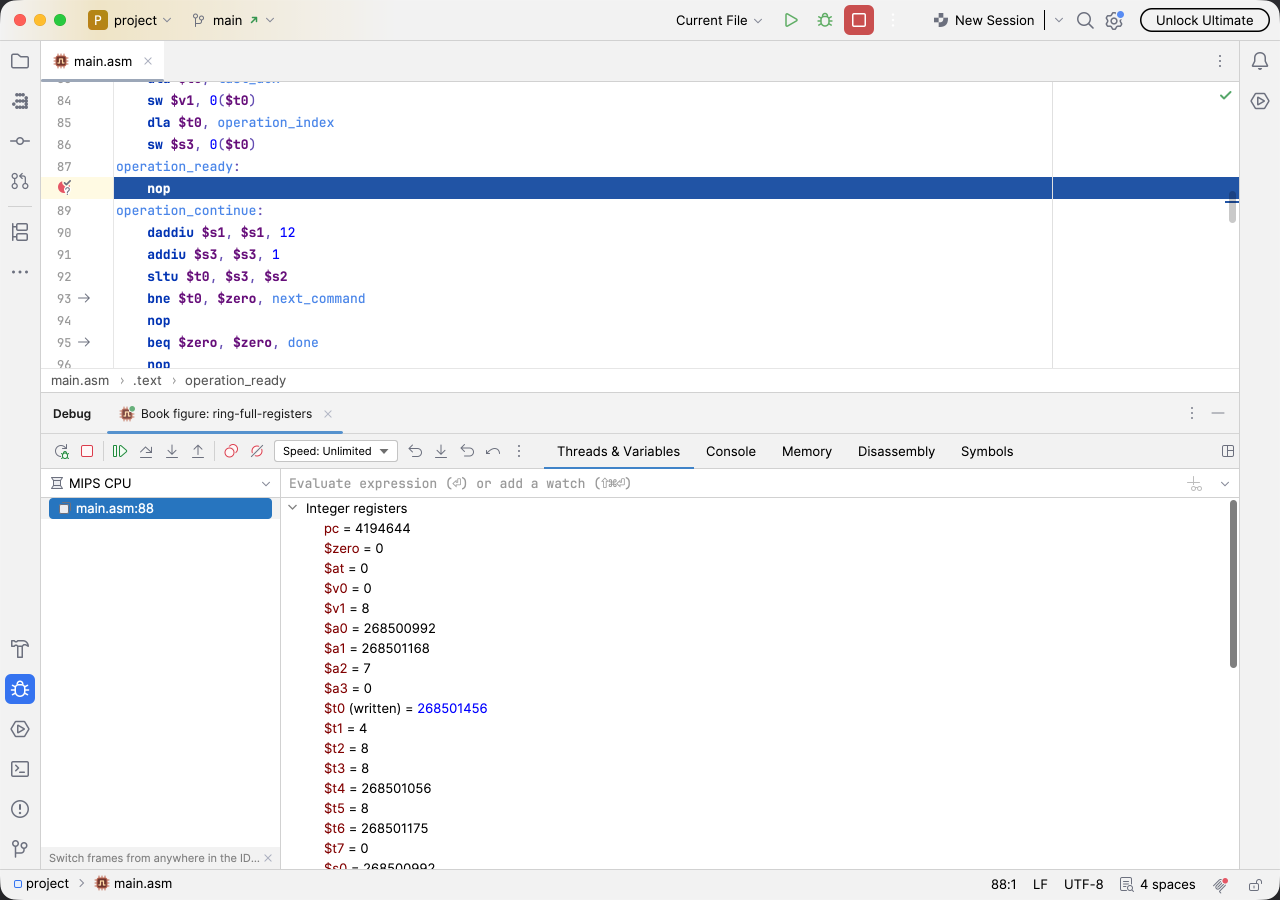
\includegraphics[artifact]{book/captures/014-ring-buffer-logger/f02-full/registers.png}}
\sbox2{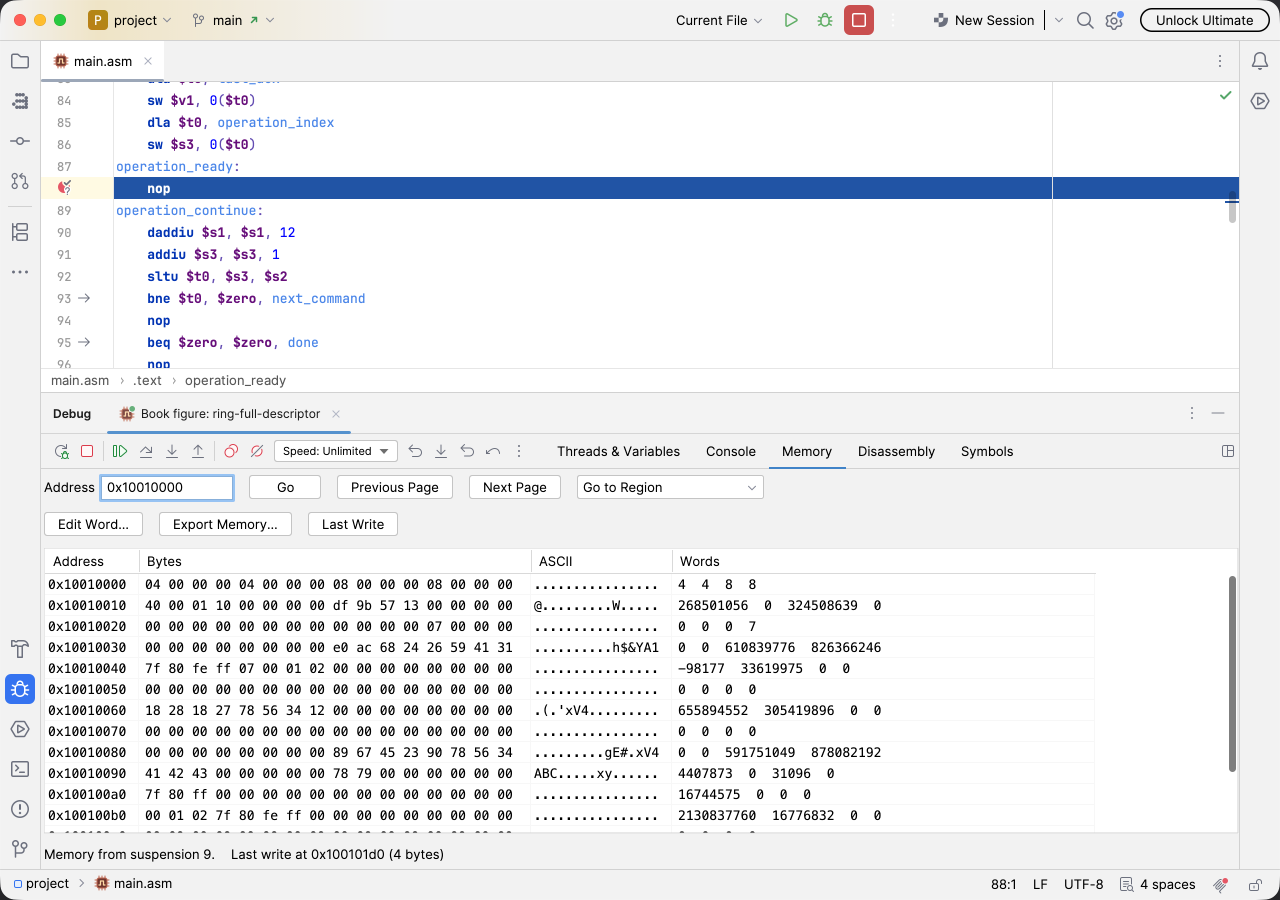
\includegraphics[artifact]{book/captures/014-ring-buffer-logger/f02-full/descriptor.png}}
\sbox4{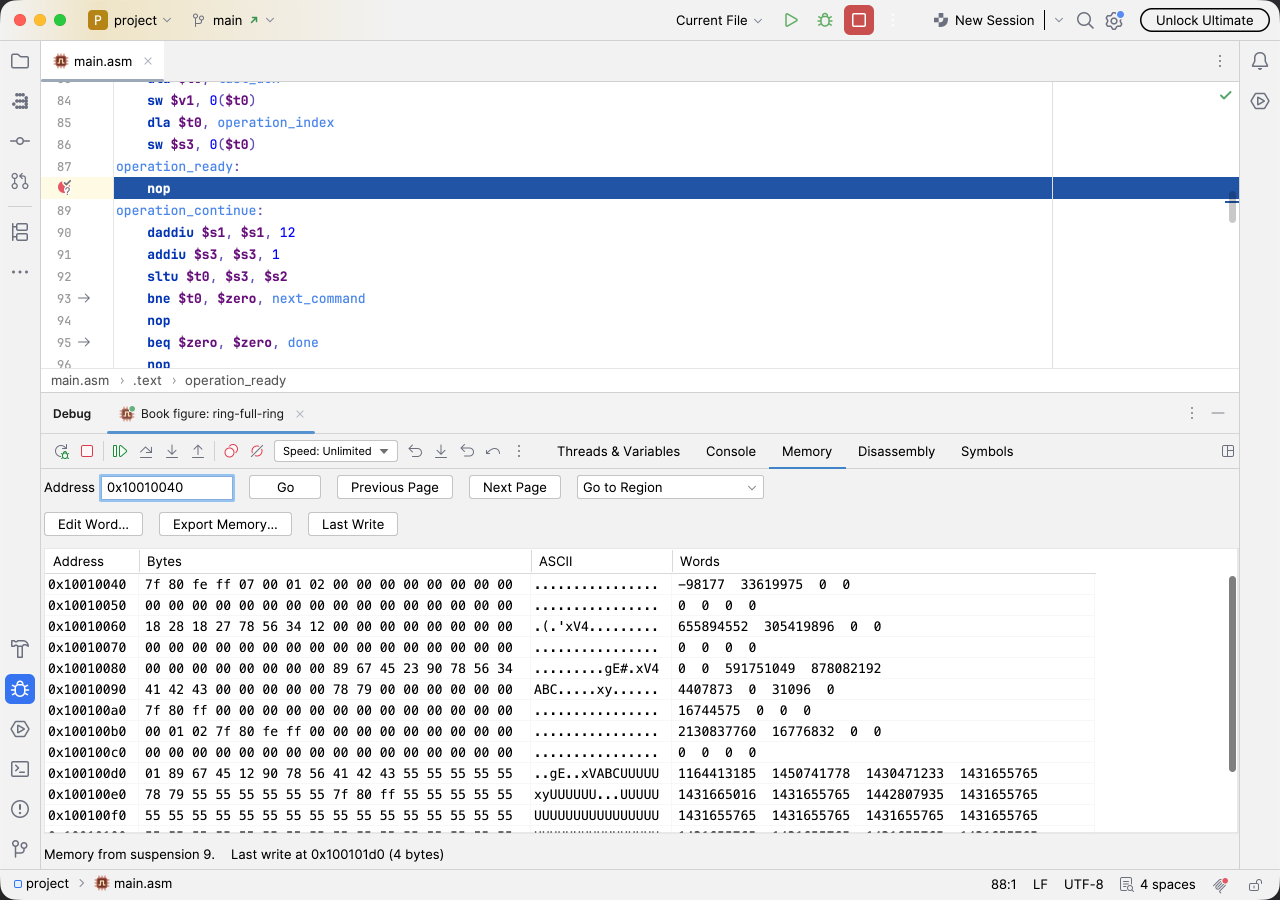
\includegraphics[artifact]{book/captures/014-ring-buffer-logger/f02-full/ring.png}}
\sbox6{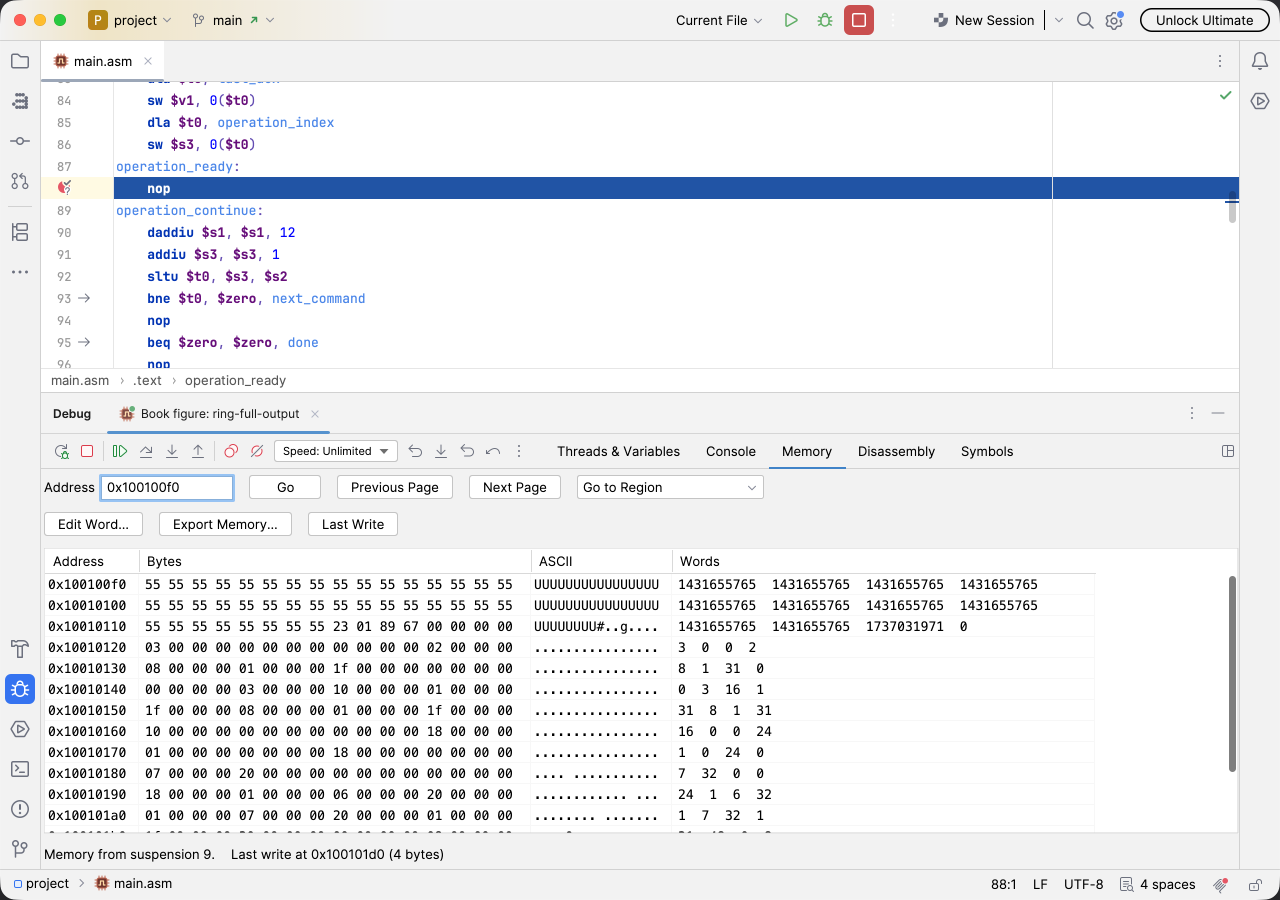
\includegraphics[artifact]{book/captures/014-ring-buffer-logger/f02-full/output.png}}
\edef\MARSringfullsourceLeft{\the\dimexpr0.036718750\wd0\relax}
\edef\MARSringfullsourceBottom{\the\dimexpr0.774444444\ht0\relax}
\edef\MARSringfullsourceRight{\the\dimexpr0.713281250\wd0\relax}
\edef\MARSringfullsourceTop{\the\dimexpr0.147777778\ht0\relax}
\edef\MARSringfullregistersLeft{\the\dimexpr0.246093750\wd0\relax}
\edef\MARSringfullregistersBottom{\the\dimexpr0.312222222\ht0\relax}
\edef\MARSringfullregistersRight{\the\dimexpr0.553906250\wd0\relax}
\edef\MARSringfullregistersTop{\the\dimexpr0.640000000\ht0\relax}
\edef\MARSringfulldescriptorLeft{\the\dimexpr0.034375000\wd2\relax}
\edef\MARSringfulldescriptorBottom{\the\dimexpr0.311111111\ht2\relax}
\edef\MARSringfulldescriptorRight{\the\dimexpr0.584375000\wd2\relax}
\edef\MARSringfulldescriptorTop{\the\dimexpr0.608888889\ht2\relax}
\edef\MARSringfullringLeft{\the\dimexpr0.034375000\wd4\relax}
\edef\MARSringfullringBottom{\the\dimexpr0.334444444\ht4\relax}
\edef\MARSringfullringRight{\the\dimexpr0.584375000\wd4\relax}
\edef\MARSringfullringTop{\the\dimexpr0.608888889\ht4\relax}
\edef\MARSringfulloutputLeft{\the\dimexpr0.034375000\wd6\relax}
\edef\MARSringfulloutputBottom{\the\dimexpr0.287777778\ht6\relax}
\edef\MARSringfulloutputRight{\the\dimexpr0.584375000\wd6\relax}
\edef\MARSringfulloutputTop{\the\dimexpr0.608888889\ht6\relax}
\begin{tikzpicture}[alt={Five annotated details after command index eight. Return status is zero and encoded size eight. Descriptor head and tail both four, used eight, capacity eight. Prefix seven at ring index four precedes payload 00 01 02 7f 80 fe ff across the end. The destination for a later pop remains filled with 55.}]
\node[anchor=north west,inner sep=0,font=\small\bfseries] (source-title) at (6mm,0) {Next instruction after publication};
\node[anchor=north west,inner sep=0] (source) at ([yshift=-1mm]source-title.south west) {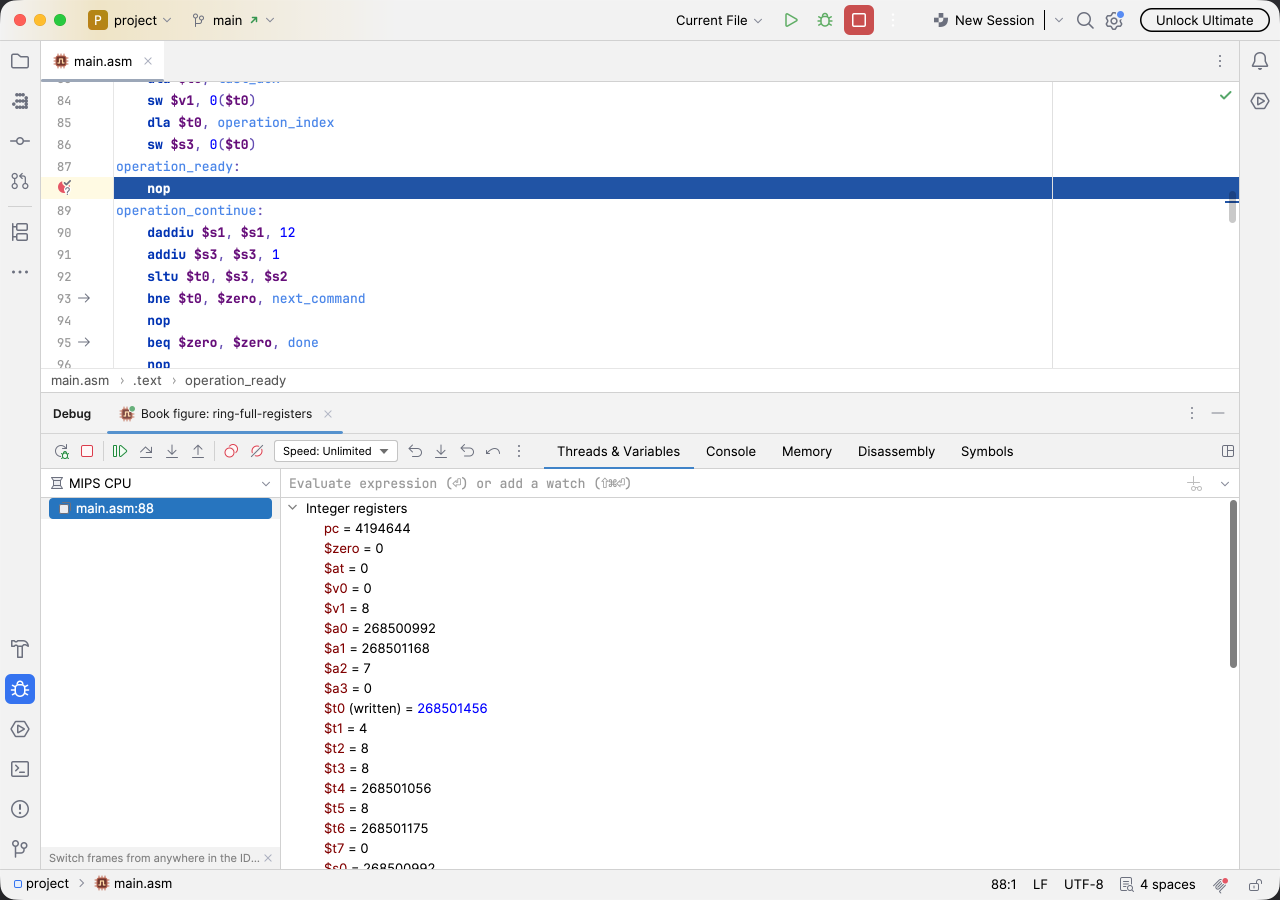
\includegraphics[width=0.54\linewidth,artifact,trim={\MARSringfullsourceLeft{} \MARSringfullsourceBottom{} \MARSringfullsourceRight{} \MARSringfullsourceTop{}},clip]{book/captures/014-ring-buffer-logger/f02-full/registers.png}};
\begin{scope}[shift={(source.south west)},x={($(source.south east)-(source.south west)$)},y={($(source.north west)-(source.south west)$)}]
\draw[black,line width=0.7pt] (0.215625000,0.057142857) rectangle (0.384375000,0.371428571);
\node[draw=black,fill=white,circle,inner sep=1.5pt,font=\footnotesize] at ($(0.215625000,0.371428571)+(-3mm,0)$) {1};
\end{scope}
\node[anchor=north west,inner sep=0,font=\small\bfseries] (registers-title) at (0.58\linewidth,0 |- source-title.north) {Signed return values};
\node[anchor=north west,inner sep=0] (registers) at ([yshift=-1mm]registers-title.south west) {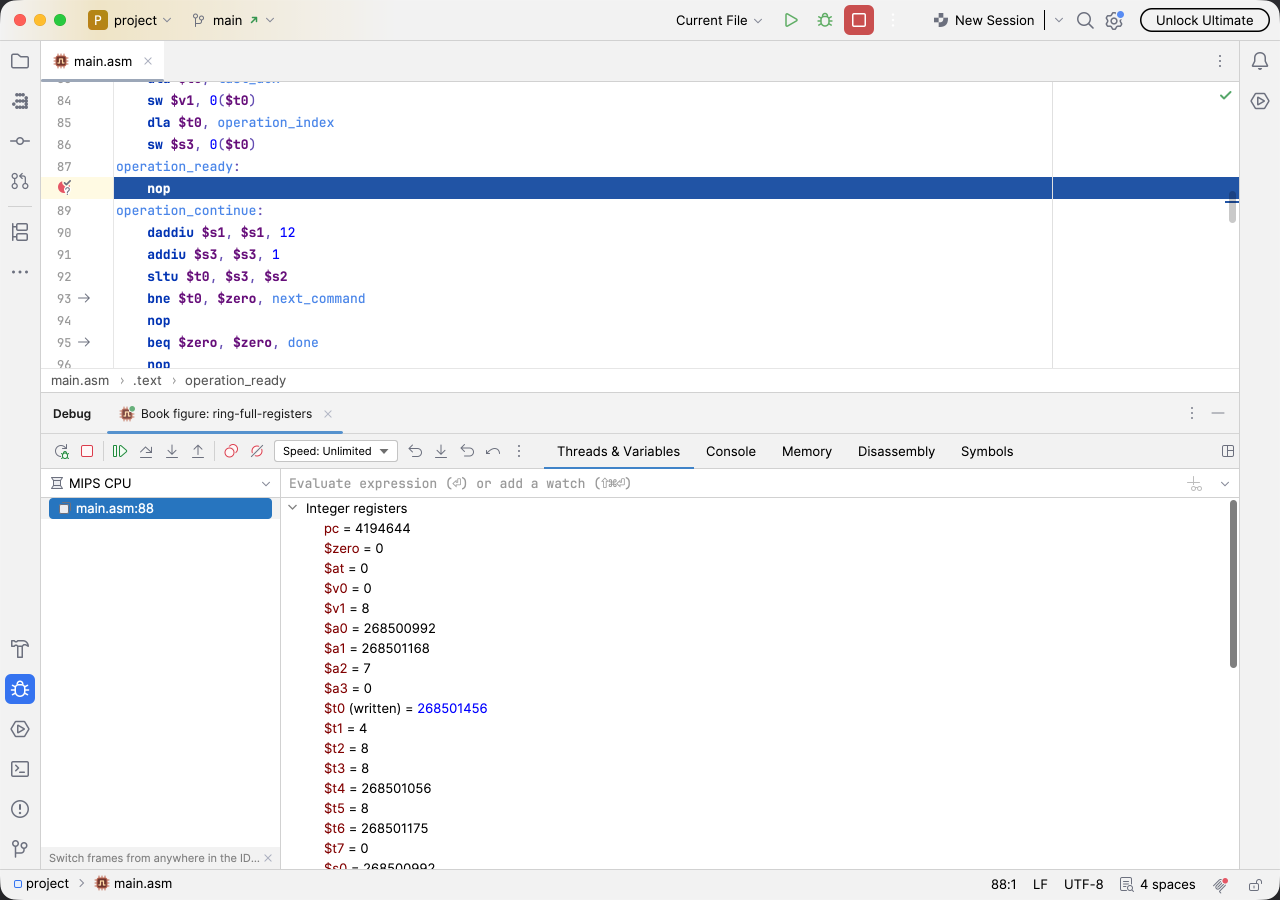
\includegraphics[width=0.42\linewidth,artifact,trim={\MARSringfullregistersLeft{} \MARSringfullregistersBottom{} \MARSringfullregistersRight{} \MARSringfullregistersTop{}},clip]{book/captures/014-ring-buffer-logger/f02-full/registers.png}};
\begin{scope}[shift={(registers.south west)},x={($(registers.south east)-(registers.south west)$)},y={($(registers.north west)-(registers.south west)$)}]
\draw[black,line width=0.7pt] (0.023437500,0.023255814) rectangle (0.226562500,0.953488372);
\node[draw=black,fill=white,circle,inner sep=1.5pt,font=\footnotesize] at ($(0.023437500,0.953488372)+(-3mm,0)$) {2};
\end{scope}
\node[anchor=north west,inner sep=0,font=\small\bfseries] (descriptor-title) at ([yshift=-3mm]source.south west) {Descriptor words and full buffer pointer};
\node[anchor=north west,inner sep=0] (descriptor) at ([yshift=-1mm]descriptor-title.south west) {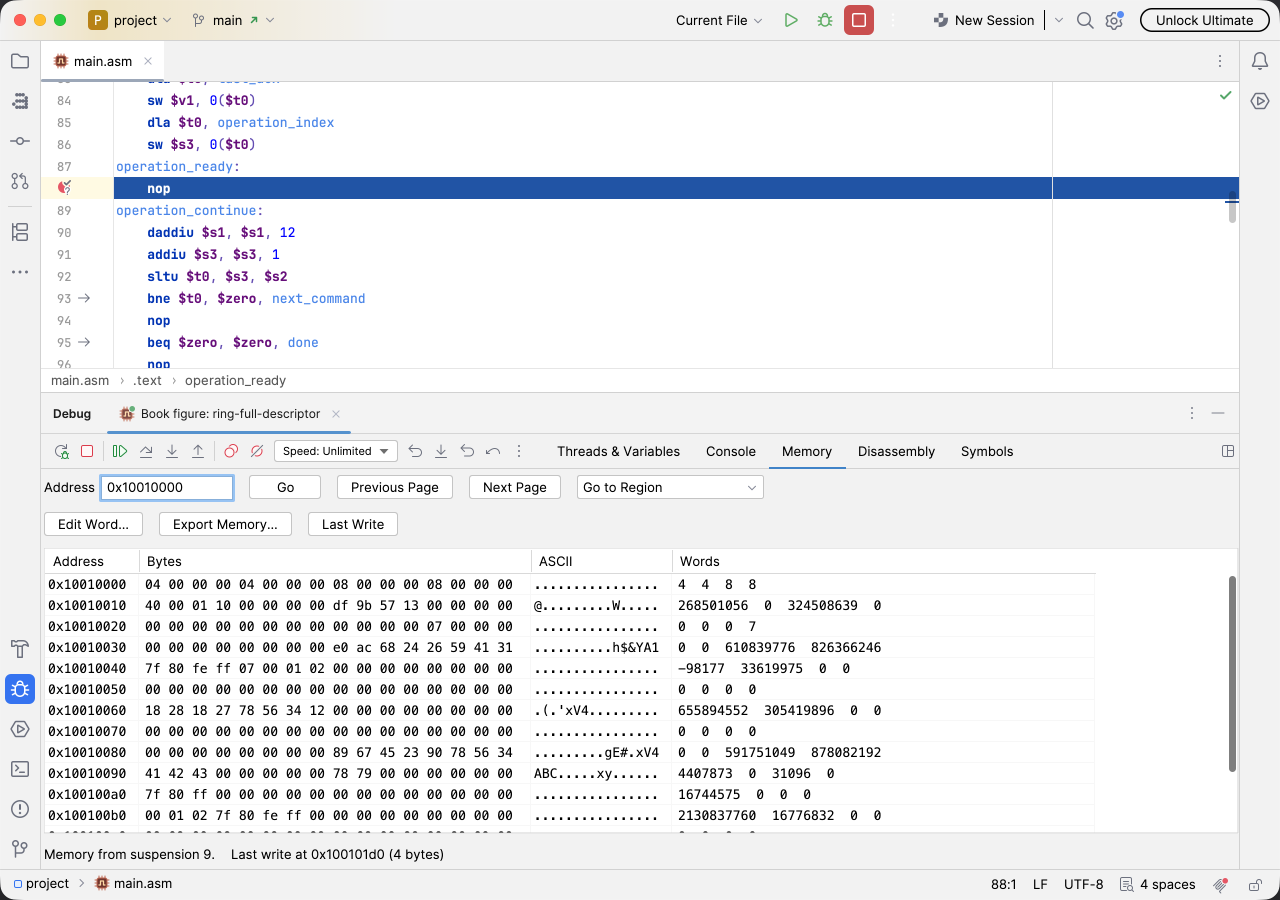
\includegraphics[width=0.84\linewidth,artifact,trim={\MARSringfulldescriptorLeft{} \MARSringfulldescriptorBottom{} \MARSringfulldescriptorRight{} \MARSringfulldescriptorTop{}},clip]{book/captures/014-ring-buffer-logger/f02-full/descriptor.png}};
\begin{scope}[shift={(descriptor.south west)},x={($(descriptor.south east)-(descriptor.south west)$)},y={($(descriptor.north west)-(descriptor.south west)$)}]
\draw[black,line width=0.7pt] (0.194672131,0.055555556) rectangle (0.997950820,0.638888889);
\node[draw=black,fill=white,circle,inner sep=1.5pt,font=\footnotesize] at ($(0,0.638888889)+(-3mm,0)$) {3};
\end{scope}
\node[anchor=north west,inner sep=0,font=\small\bfseries] (ring-title) at ([yshift=-3mm]descriptor.south west) {Physical ring bytes, including mapped padding};
\node[anchor=north west,inner sep=0] (ring) at ([yshift=-1mm]ring-title.south west) {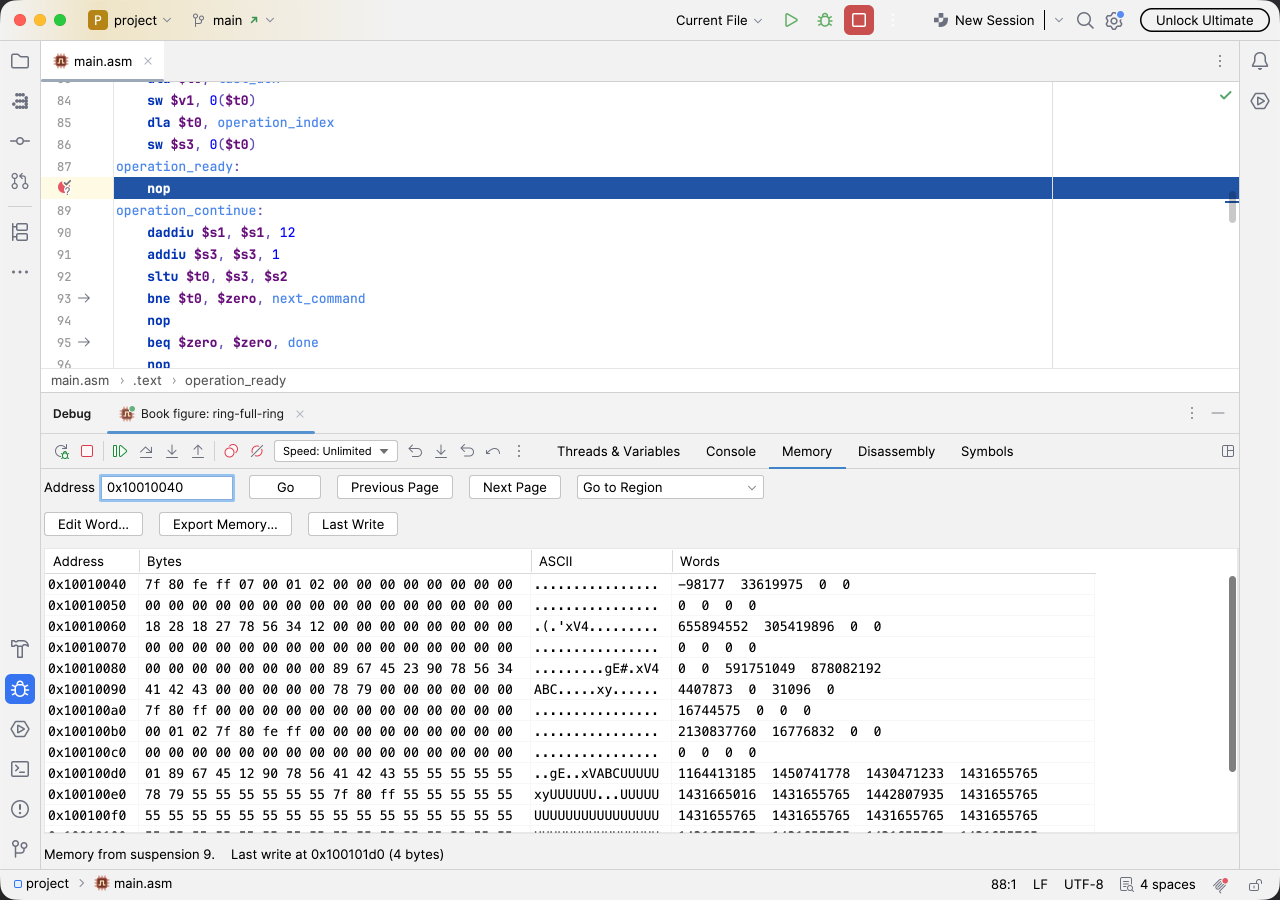
\includegraphics[width=0.84\linewidth,artifact,trim={\MARSringfullringLeft{} \MARSringfullringBottom{} \MARSringfullringRight{} \MARSringfullringTop{}},clip]{book/captures/014-ring-buffer-logger/f02-full/ring.png}};
\begin{scope}[shift={(ring.south west)},x={($(ring.south east)-(ring.south west)$)},y={($(ring.north west)-(ring.south west)$)}]
\draw[black,line width=0.7pt] (0.194672131,0.078431373) rectangle (0.997950820,0.490196078);
\node[draw=black,fill=white,circle,inner sep=1.5pt,font=\footnotesize] at ($(0,0.490196078)+(-3mm,0)$) {4};
\end{scope}
\node[anchor=north west,inner sep=0,font=\small\bfseries] (output-title) at ([yshift=-3mm]ring.south west) {Output bytes and neighboring objects};
\node[anchor=north west,inner sep=0] (output) at ([yshift=-1mm]output-title.south west) {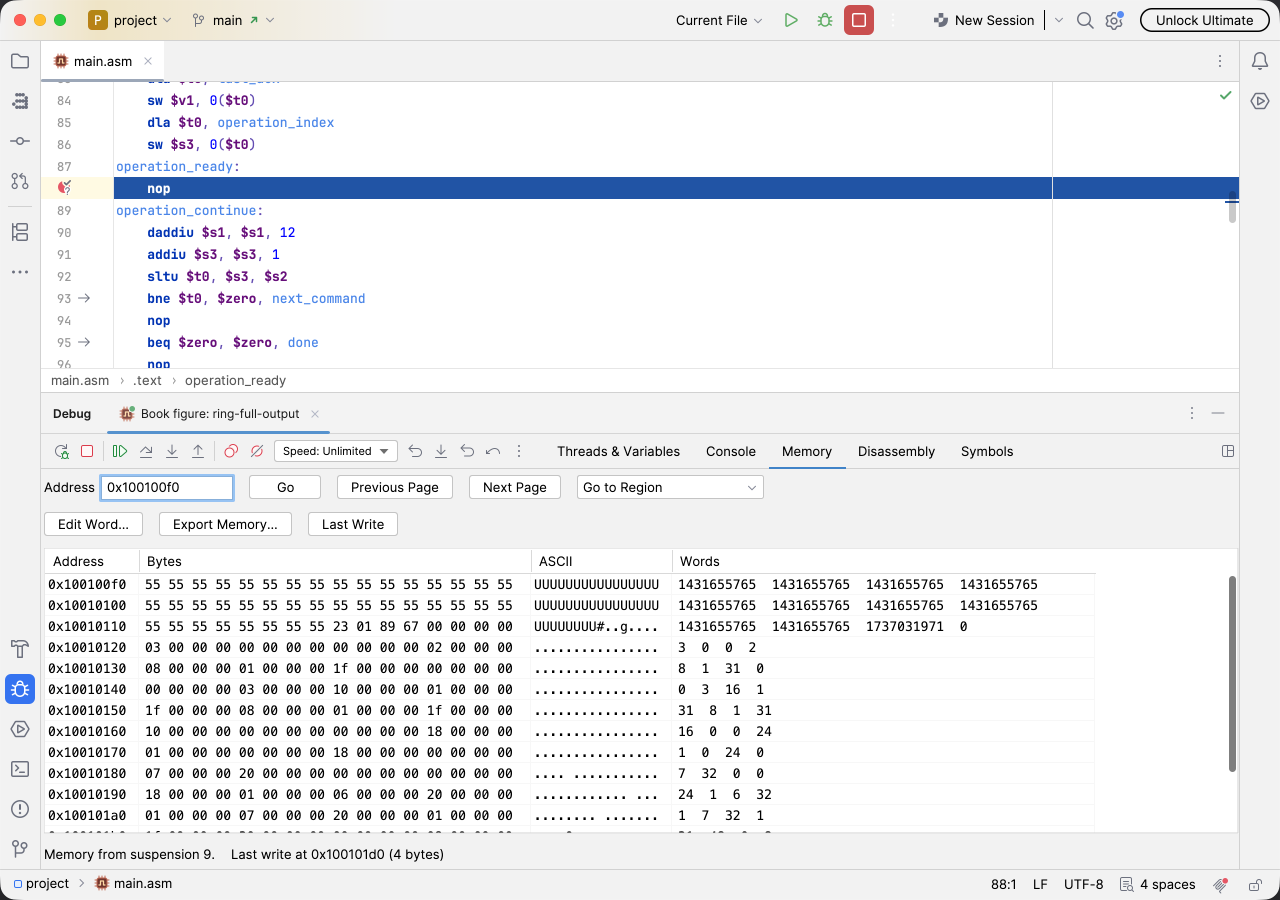
\includegraphics[width=0.84\linewidth,artifact,trim={\MARSringfulloutputLeft{} \MARSringfulloutputBottom{} \MARSringfulloutputRight{} \MARSringfulloutputTop{}},clip]{book/captures/014-ring-buffer-logger/f02-full/output.png}};
\begin{scope}[shift={(output.south west)},x={($(output.south east)-(output.south west)$)},y={($(output.north west)-(output.south west)$)}]
\draw[black,line width=0.7pt] (0.194672131,0.043010753) rectangle (0.997950820,0.720430108);
\node[draw=black,fill=white,circle,inner sep=1.5pt,font=\footnotesize] at ($(0,0.720430108)+(-3mm,0)$) {5};
\end{scope}
\end{tikzpicture}
\par\smallskip
\begin{minipage}{\linewidth}
\small
\begin{enumerate}
\setlength{\itemsep}{2pt}
\setlength{\parsep}{0pt}
\item This stop follows command index 8, the ninth command: push a seven-byte payload into an empty capacity-eight ring whose cursors were already at index 4. Earlier commands have removed the previous records, including an empty record. The next instruction remains \texttt{operation\_ready}.
\item \texttt{\$v0 = 0} reports success and \texttt{\$v1 = 8} reports the encoded size. Seven payload bytes and one prefix consume the entire capacity. The exact fit is accepted; this representation reserves no sentinel slot.
\item The descriptor words are now $[4,4,8,8]$: head, tail, used and capacity. Equal cursors describe a full ring because used equals capacity. An empty ring can have the same cursors but used zero. The unchanged doubleword at offset 16 still points to \texttt{0x10010040}.
\item At index 4, prefix \texttt{07} begins the queued record. Read forward circularly: payload \texttt{00 01 02} occupies indices 5 through 7, then \texttt{7f 80 fe ff} occupies indices 0 through 3. Every one of the first eight bytes is occupied. The zero bytes beyond index 7 are mapped padding outside this queue.
\item The later pop destination starts at output plus 32, address \texttt{0x100100f8}, eight bytes into the first displayed row. Its bytes remain \texttt{55}; push writes the ring, not this destination. The final row also includes \texttt{output\_end} and the start of the command table, which are separate objects.
\end{enumerate}
\end{minipage}
\caption{An exact-fit record fills all eight bytes even though head and tail are equal.}
\label{capture:014-ring-buffer-logger-f02-full}
\label{ring-f02-full}
\end{figure}
\par
